This chapter presents the design of a safe controller for the  robotic patient manipulator in 3D Cartesian space, where the unsafe region is defined as an ellipsoid with static boundaries, i.e. fixed in space with respect to time. The unsafe region is defined such that it is within the reach of the instrument tip. It is desired to construct the unsafe area such that the interior of the ellipsoid is unsafe, thus representing a heart or another vital sensitive organ which can not be cut under no circumstances.
\begin{figure}[H]
\centering
\subbottom[The Robotic patient manipulator.]{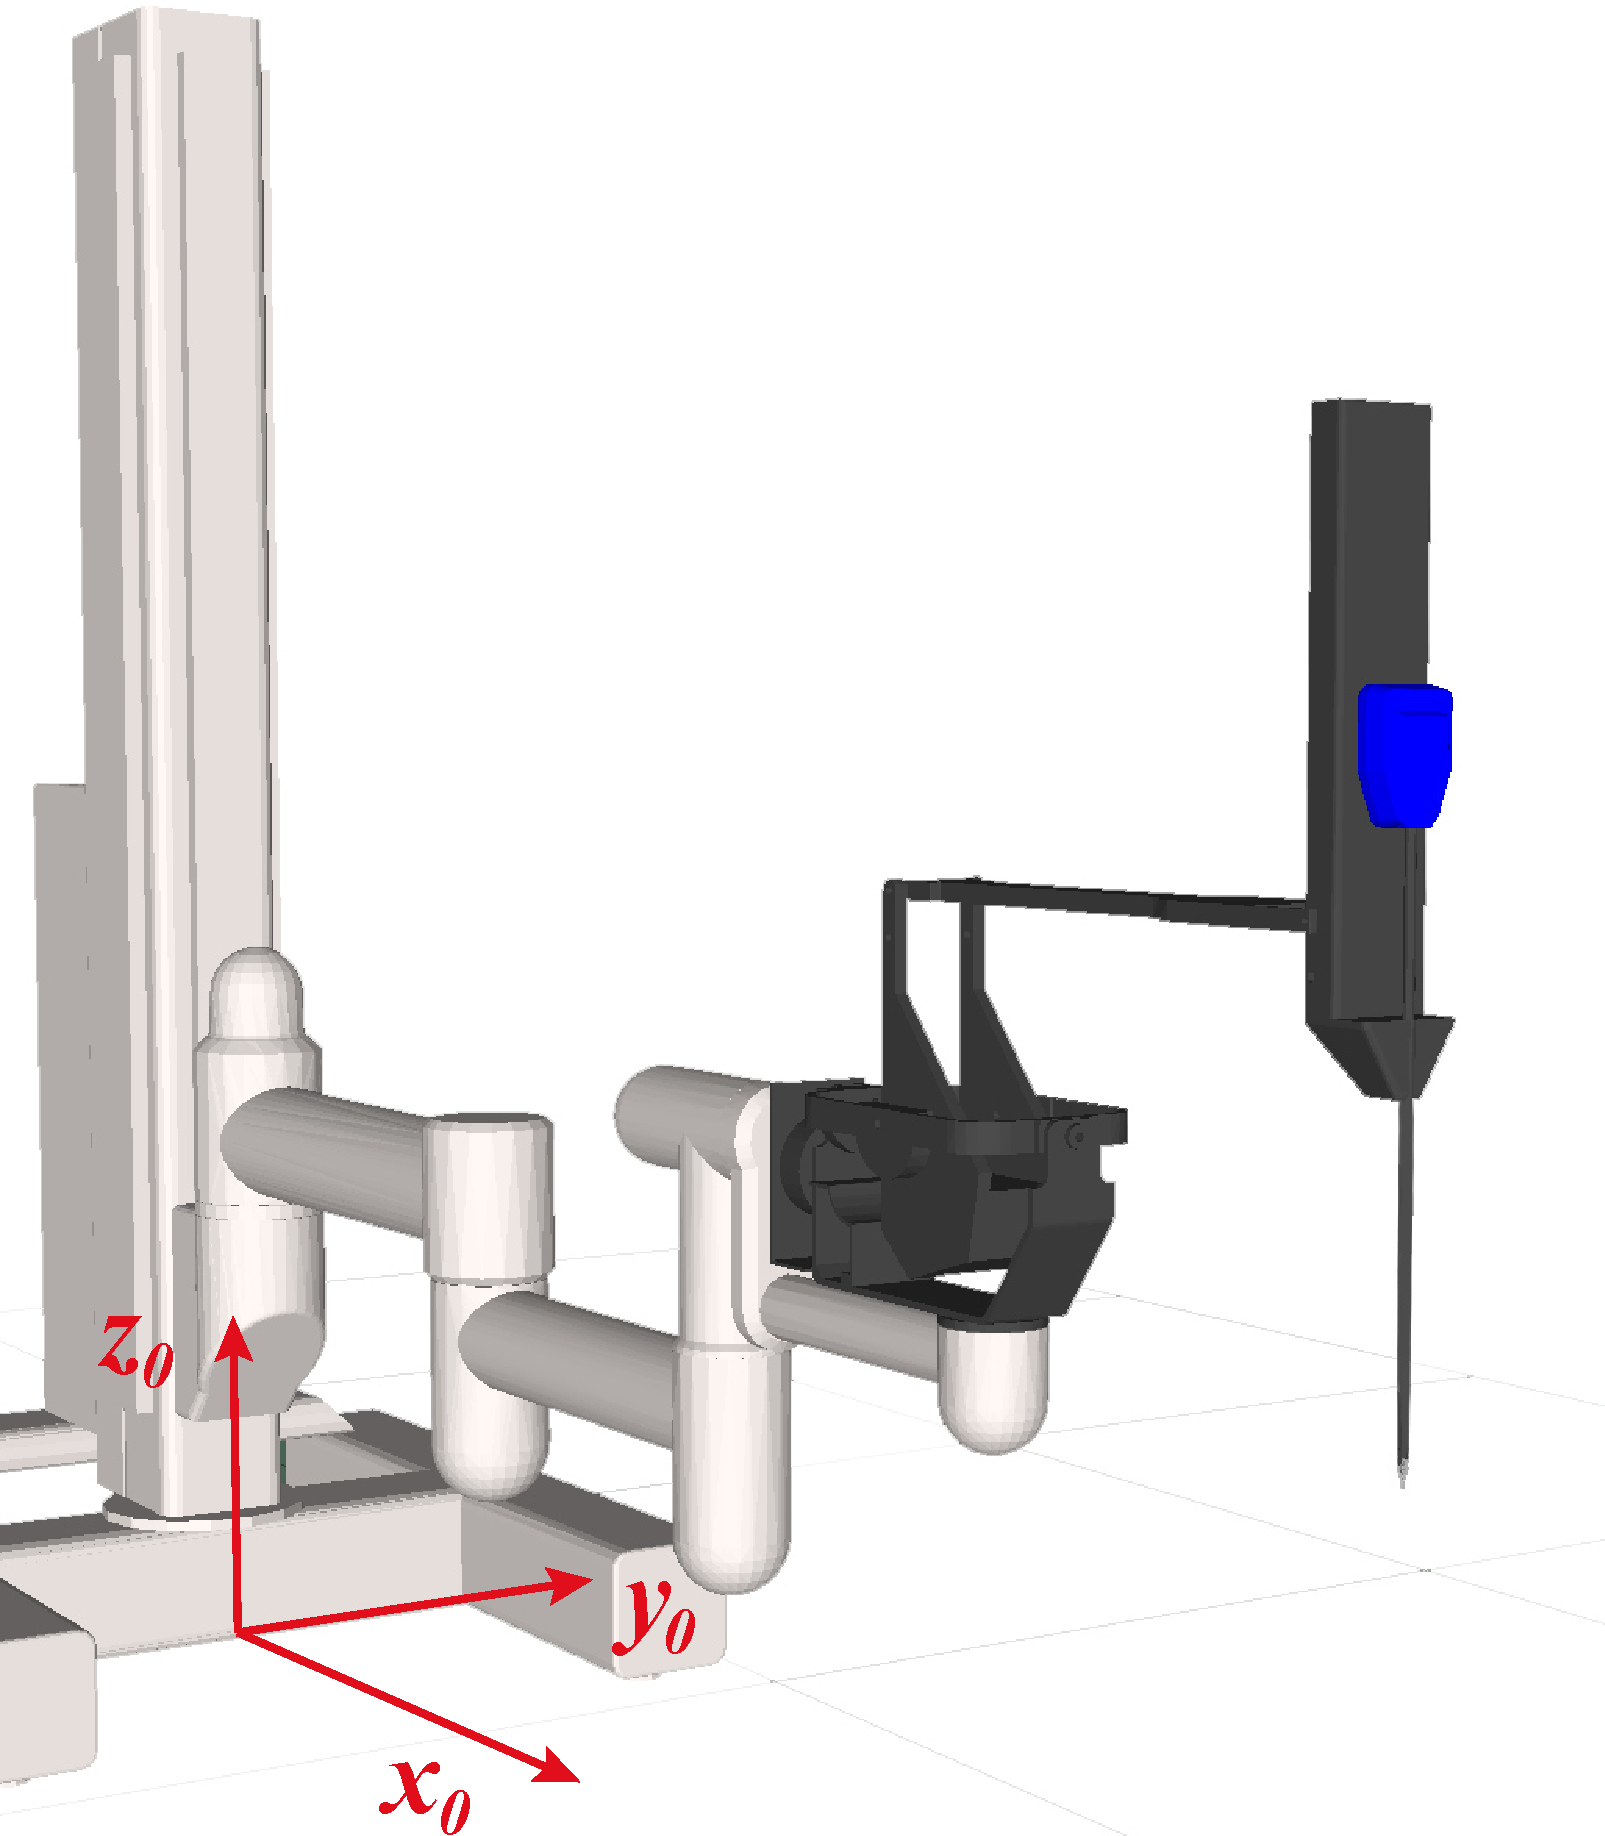
\includegraphics[width=0.45\textwidth]{rviz_09_17_18_frame1.pdf}\label{fig:rviz_09_17_18_frame}}%
	\hspace*{5mm}
\subbottom[The robot hand and instrument.]{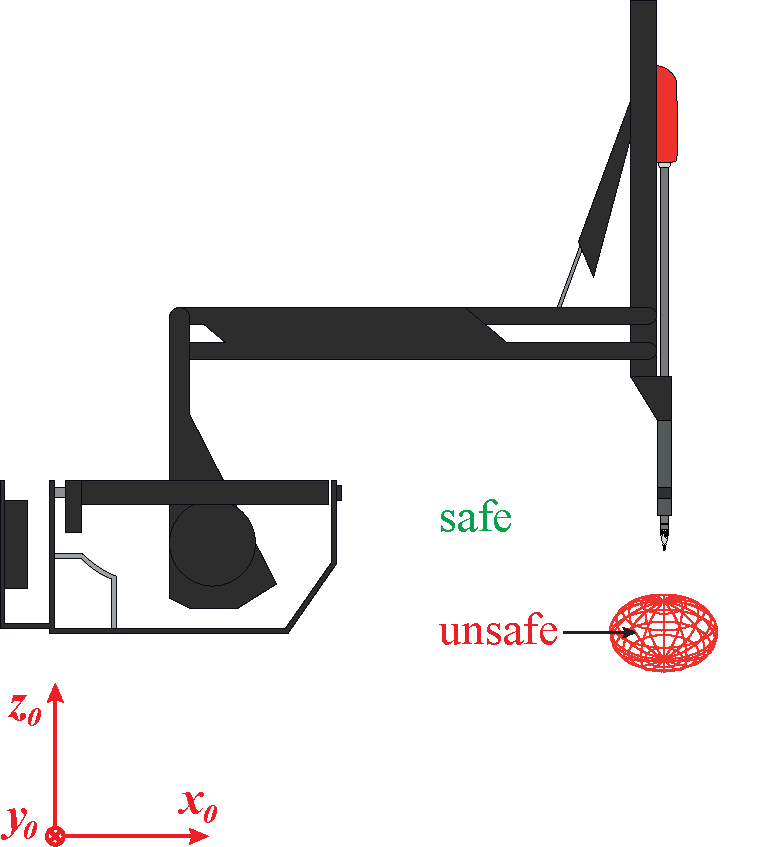
\includegraphics[width=0.45\textwidth]{robot_hand_unsafe_region.pdf}\label{fig:robot_hand_unsafe_region}}%
\caption{Patient manipulator and a fixed region within the reachable space $\mathcal{X}$ that is unsafe, $\mathcal{X}_u$, marked by a red ellipsoid thus insinuating an ellipsoid as \gls{cbf}.}
\label{fig:robot_hand_3d}
\end{figure}
Given the reachability of the robotic end effector which is tested to be roughly a square with the measures [0.2 0.2 0.2]\,m centered in (0,0,0), the sets considered in this chapter can be outlined in \autoref{tab:intervals_3d}.
\begin{table}[H]
	\begin{tabularx}{\textwidth}{X X X X}
\rowcolor{HeaderBlue} 
$\mathcal{X}$ & $\mathcal{X}_u$  & $\mathcal{X}_0$ & $\mathcal{T}$ \\
$\mathcal{X} = \{ x \in  [-\bar{\Lambda}_\text{lim}, \bar{\Lambda}_\text{lim}] $,\newline $ {\color{white}{mmm}} y \in [-\bar{\Lambda}_\text{lim}, \bar{\Lambda}_\text{lim}] $,\newline ${\color{white}{mmm}} z \in  [-\bar{\Lambda}_\text{lim}, \bar{\Lambda}_\text{lim}] \}$ & 
$\mathcal{X}_u$ consist of an ellipsoid with semi-axes $r_x,r_y,r_z$. &  $\mathcal{X}_u^c = \mathcal{X} \backslash \mathcal{X}_u $& $\mathcal{T}$ consist of a layer around the ellipsoid with $\text{thickness}=1$.\\
\end{tabularx}
\caption{Sets considered in this chapter, where $r_x=0.03$\,m, $r_y=0.06$\,m, $r_z=0.03$\,m are lengths of the semi-axes of an ellipsoid and $\bar{\Lambda}_\text{lim}=0.1$m being the extremity of the box encircling the reachable space.}
\label{tab:intervals_3d}
\end{table}
%
The theory, analysis and implementation aspects presented in this chapter differs from the previous work in this report. In contrast to \autoref{chap:cbf_1d_static} and \autoref{chap:cbf_1d_dynamic}, which solely comprise the prismatic slide joint, this chapter concerns the five independent revolute joints as well. Accordingly, this chapter presents the material required to be able to manoeuvre in the 3D Cartesian space and to be able to specify an unsafe set $\mathcal{X}_u$ encircled by an ellipsoid. This implies the topics:
\begin{itemize}
\item Development of a sufficient model describing movement in three dimensions.
\item Construction of a control barrier function fulfilling the demand for an ellipsoid encirclement of $\mathcal{X}_u$.
\item Development of the control system.
\item Implementation in MATLAB.
\item Implementation on the Da Vinci robot. This entails a kinematic description of the robot links and joints such that a translation between the 3D Cartesian space and the 6D joint space can be established.
\end{itemize}
Thus the first topic will be to model the movement sufficiently.
\section{Modelling of Robot Hand Movement in 3D}
The system shall be modelled as a linear state space system on the form:
\begin{flalign*}
\dot{\textbf{x}} &= \textbf{A}\,\textbf{x} + \textbf{B}\,\textbf{u} \\
\textbf{y} &= \textbf{C}\textbf{x}
\end{flalign*}
%In order to set up a dynamic model of the da Vinci robot hand, a decision is made to model the three axes as decoupled for initial simplification. \textcolor{red}{Argue why, something about measurement, as movements are composed from changing joint angles obviously the axes are coupled, but it is also dependent on the low level controllers on the FPGA.} Measurements are made for a step input on each of the three axes, as shown in \textcolor{red}{FIGURE}
The movement en the three dimensional space may be modelled as three decoupled systems. While there may be coupling between the systems, the decoupling simplifies the modelling phase significantly and it is still a realistic version of the real scenario.
%
%\textcolor{red}{Make measurement of step for cases: x-axis, y-axis, z-axis, and xyz at the same time. Compare to slide measurement.}
%
%It is decided to model the response for each of the three (decoupled) axes as three first order systems, and the open loop system for the robot hand is formulated as:
\begin{equation}\label{eq:3D_sys_static_openloop}
\dot{\mathbf{x}}=
\dot{\begin{bmatrix}
x_x\\x_y\\x_z
\end{bmatrix}} =
\underbrace{\begin{bmatrix}
-1/\tau_x & 0 & 0\\0 & -1/\tau_y & 0 \\ 0 & 0 & -1/\tau_z
\end{bmatrix}
\begin{bmatrix}
x_x\\x_y\\x_z
\end{bmatrix}}_{f(\mathbf{x})} +
\underbrace{\begin{bmatrix}
1/\tau_x& 0 & 0 \\ 0& 1/\tau_y & 0 \\0& 0& 1/\tau_z
\end{bmatrix}}_{g(\mathbf{x})}
\mathbf{u}
\end{equation}
\begin{tabular}{rp{12.5cm}} 
where  &  \\
$x_x$ & is the position in the $x$-axis \\
$x_y$ & is the position in the $x$-axis \\
$x_z$ & is the position in the $x$-axis \\
$\tau_x$ & is the time constant associated with a step purely in the $x$-axis \\
$\tau_y$ & is the time constant associated with a step purely in the $y$-axis \\
$\tau_z$ & is the time constant associated with a step purely in the $z$-axis 
\end{tabular}\\

The time constants are measured from \textcolor{red}{appendix ??} and found to:
\begin{flalign*}
\tau_x = 0.110\,\text{s} \mm , \mm \tau_y = 0.110\,\text{s} \mm , \mm \tau_z = 0.110\,\text{s}
\end{flalign*}
With a sufficient model established the \gls{cbf} can be considered.
\section{Construction of CBF}
A \gls{cbf} is proposed that complies with the first two constraints in \autoref{def:barrier_certificate}, i.e. a function that is positive on the set $\mathcal{X}_u$ and nonpositive on the set $\mathcal{X}_0$. In order to make sure that the robot tool will not penetrate the heart or another desired three dimensional region, the unsafe set $\mathcal{X}_u$ is defined as an ellipsoid. This ellipsoid enclosing the region $\mathcal{X}_u$ as visualized in \autoref{fig:robot_hand_unsafe_region}, must be the zero level set of the CBF. The CBF is proposed of the form:
\begin{equation}
	B(\mathbf{x}) = -\left(  \left(\frac{x_x-c_x}{r_x}\right)^2 + \left(\frac{x_y-c_y}{r_y}\right)^2 + \left(\frac{x_z-c_z}{r_z}\right)^2 - 1 \right)\label{eq:barrier_3d}
\end{equation}
\begin{tabular}{rl}
	where&\\
	$[c_x\,\, c_y\,\, c_z]$ & is the coordinate of the center of the ellipsoid, $\mathbf{c}\in\mathbb{R}^3$ \\
	$[r_x\,\, r_y\,\, r_z]$ & is the lengths of the semi-axes of the ellipsoid, $\mathbf{r}\in\mathbb{R}^3_+$ \\
\end{tabular}\\

The \gls{cbf} is visualized in \autoref{fig:zerolevelset_3d}. The zero level set enclosing the unsafe region $\mathcal{X}_u$ shown as a red ellipsoid, the one level set shown in black. Note that the function $-B(\mathbf{x})$ will have the same zero level set, but have positive values outside the ellipsoid, indicating that it is the safe area $\mathcal{X}_0$ that is enclosed by the ellipsoid.
\vspace{-0.5cm}
\begin{figure}[H]
\centering
	\hspace*{-3cm}
	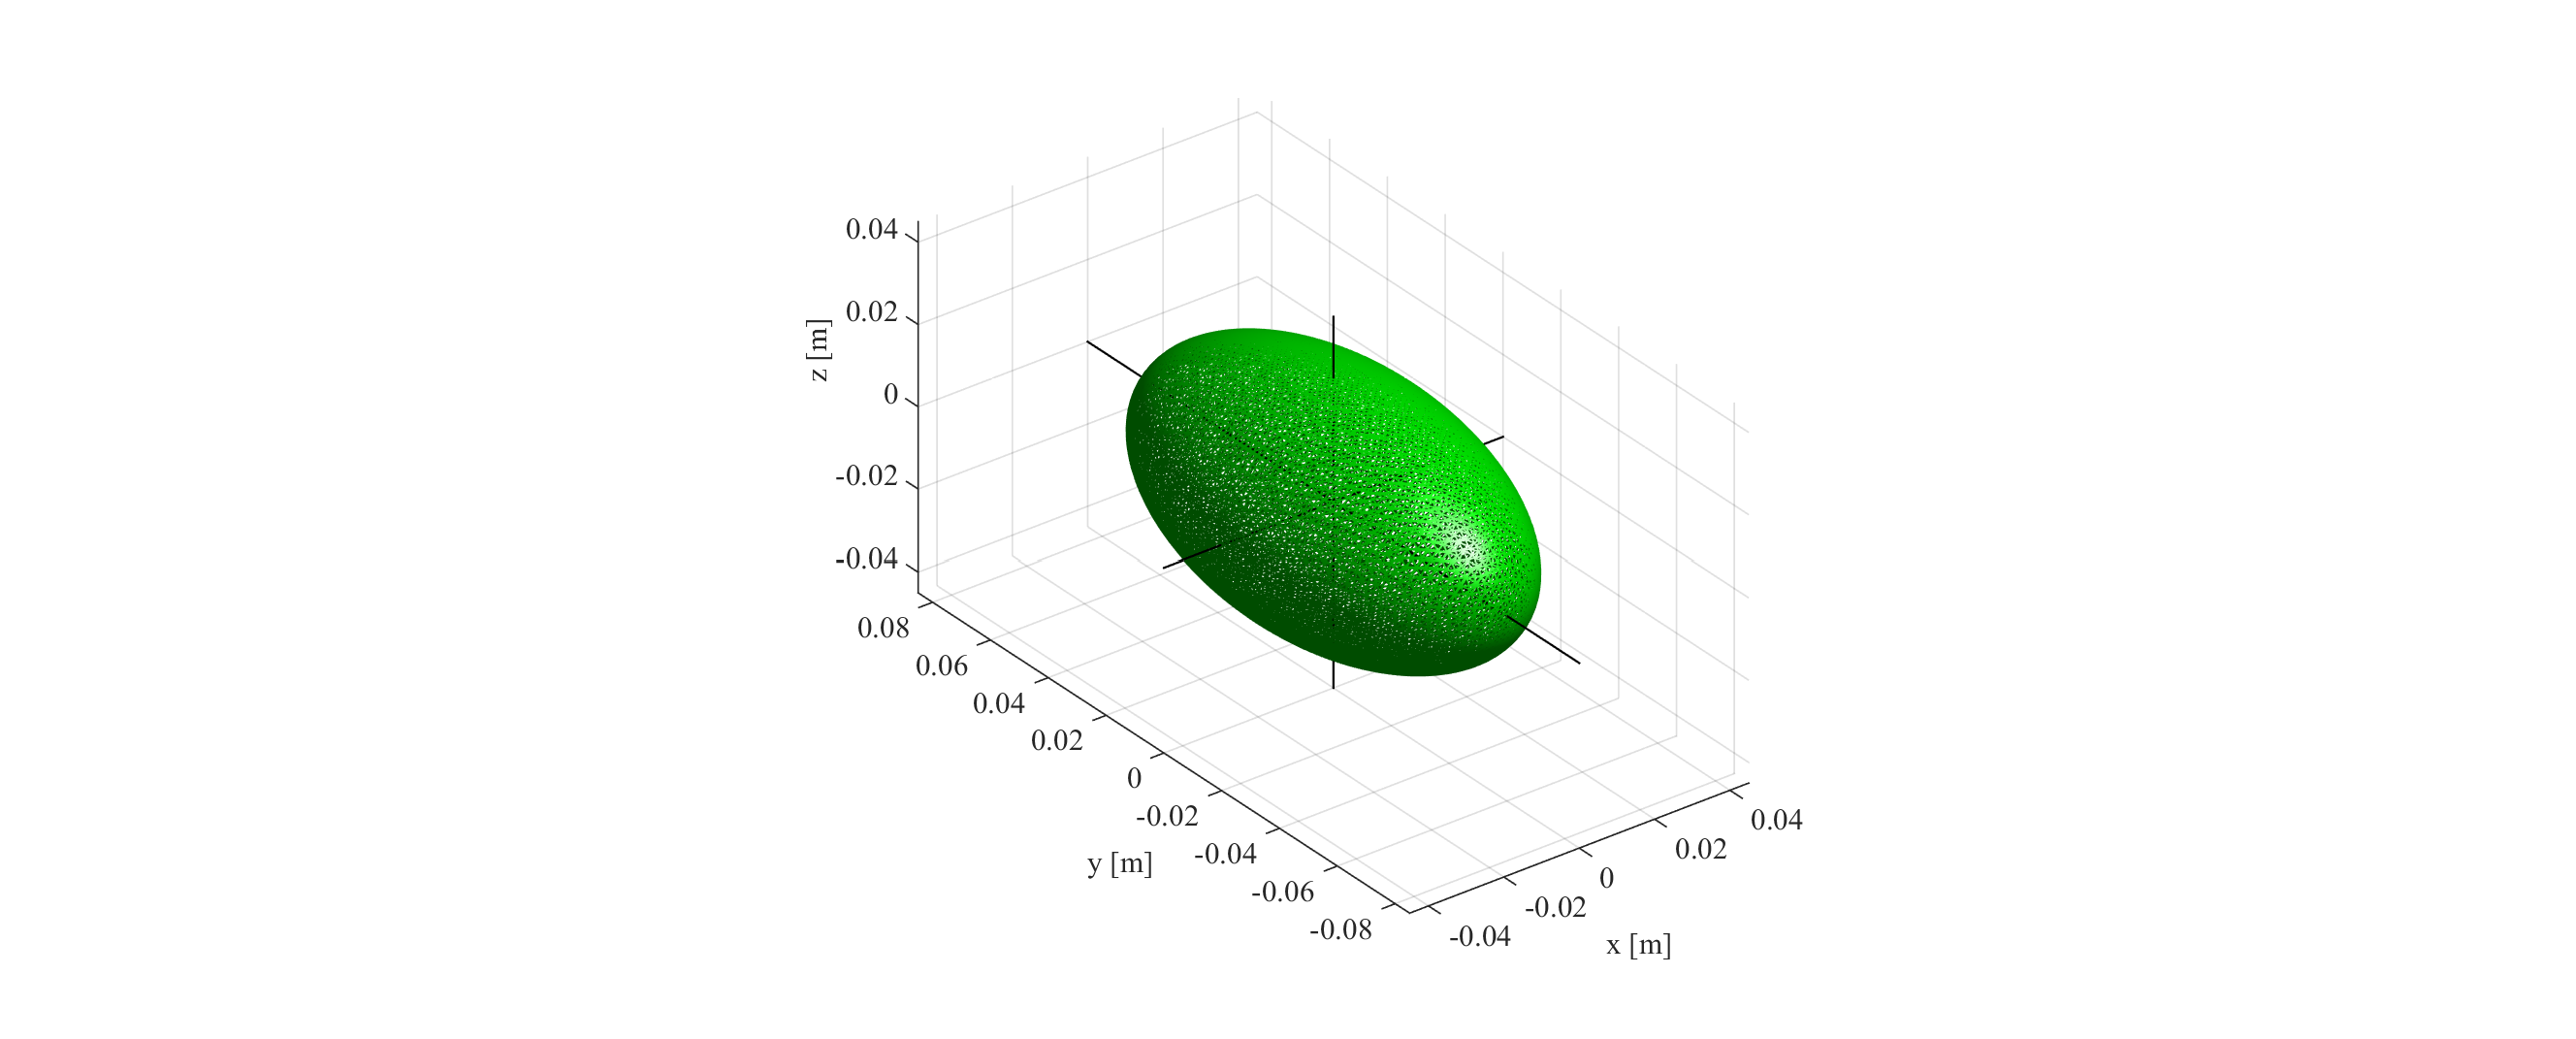
\includegraphics[width=1.3\textwidth]{cbf_3d_init.eps}
	\caption{CBF on the form described in with center $\mathbf{c}= [0,\,\,\,\, 0,\,\,\,\, 0]$ and $\mathbf{r}=[0.03,\,\,\,\, 0.05,\,\,\,\, 0.03]$.}
	\label{fig:zerolevelset_3d}
\end{figure}
%
%\begin{figure}[H]
%	\centering
%	\hspace*{-15mm}
%	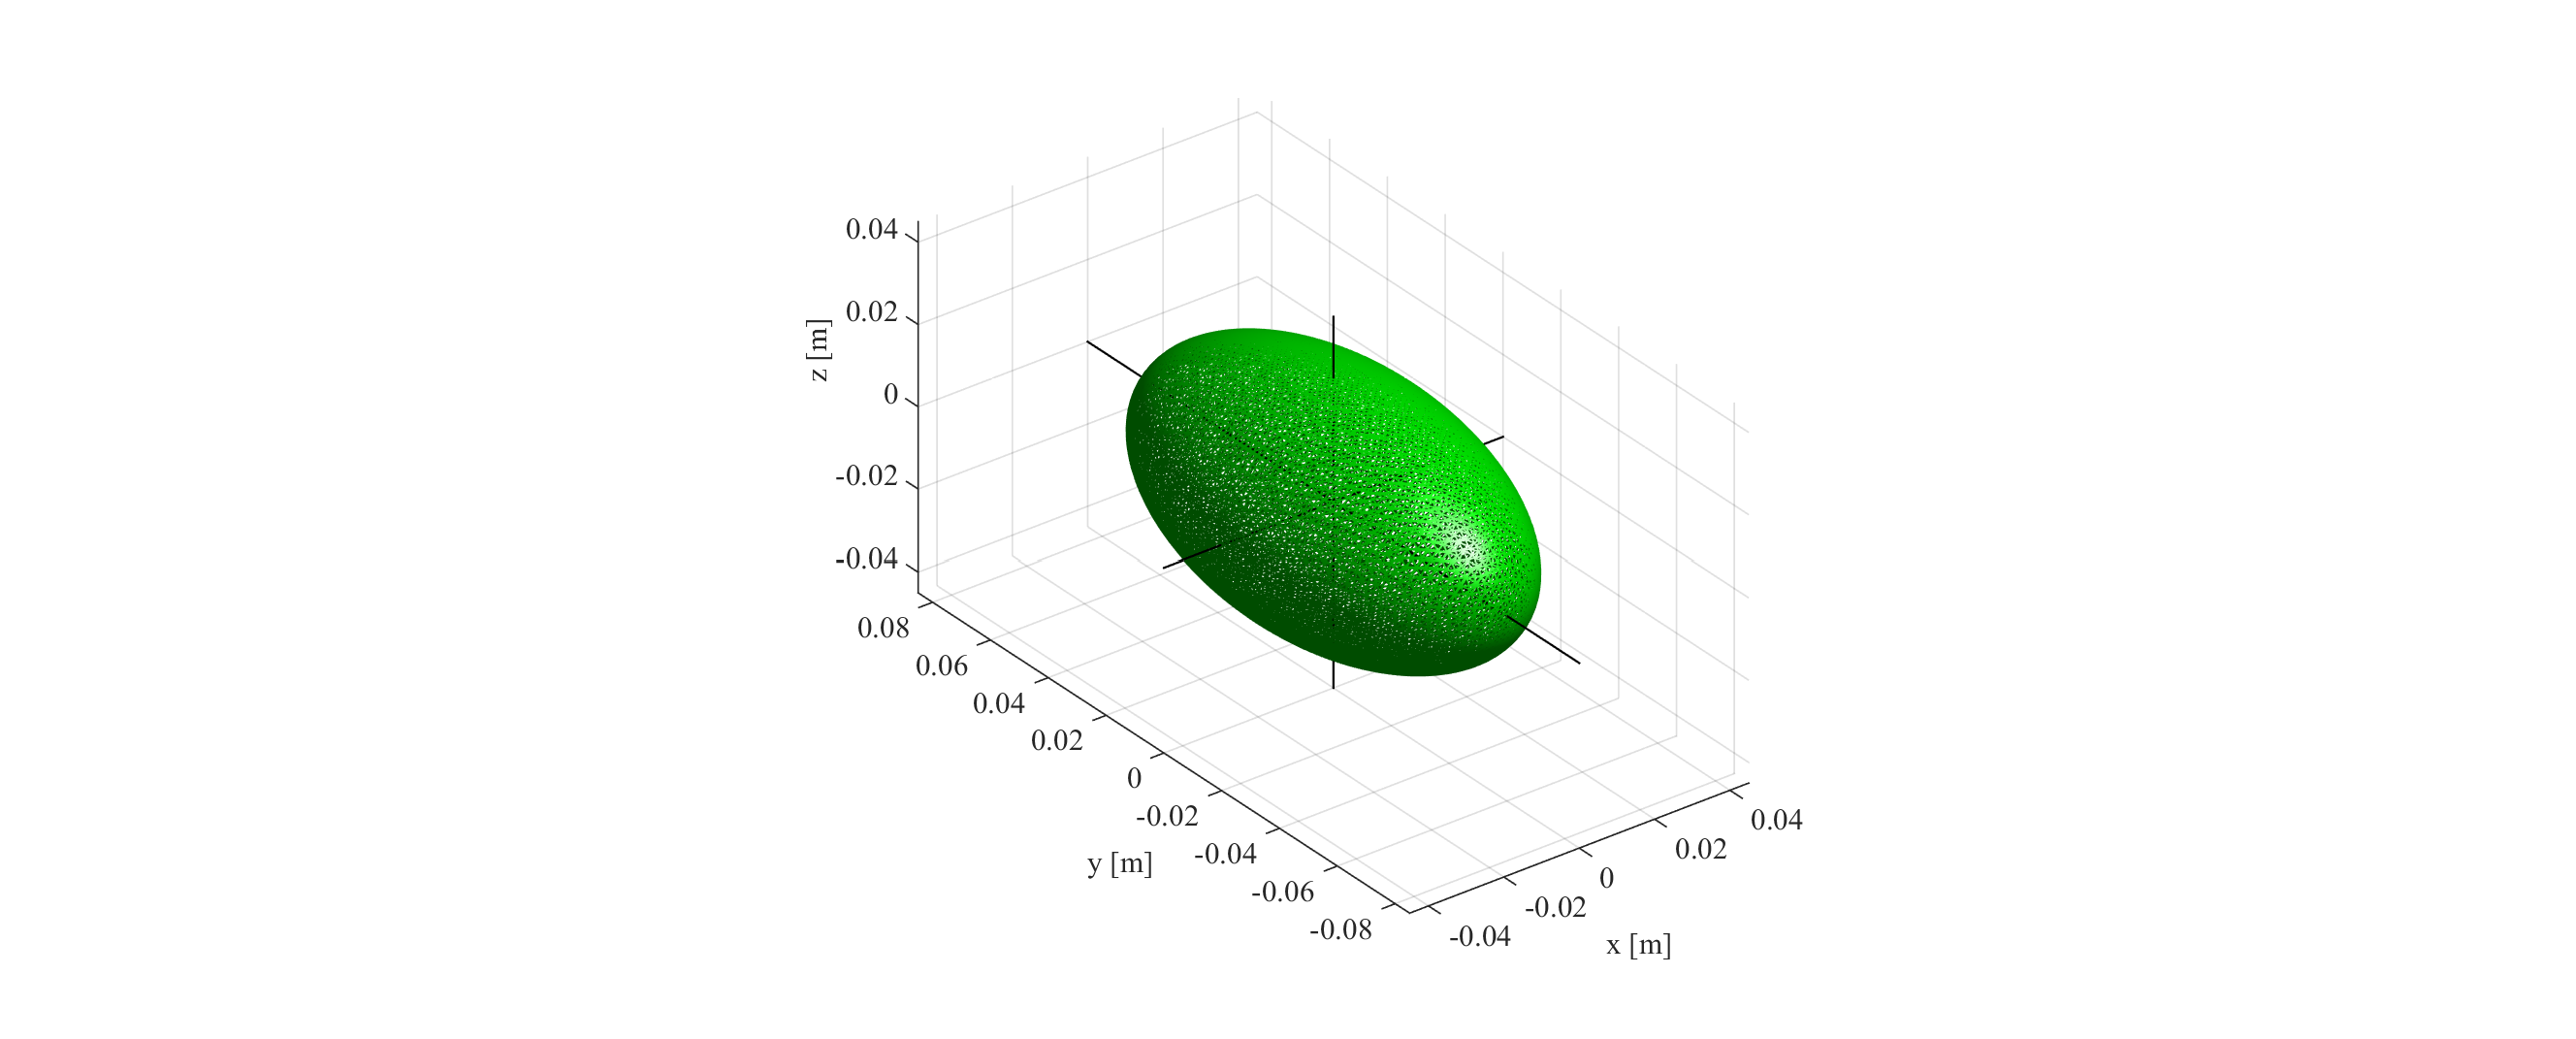
\includegraphics[width=1.2\textwidth]{cbf_3d_init.eps}
%	\caption{Example of a CBF on the form described in \autoref{eq:barrier_3d}, here with $\mathbf{c}= [0.1,\,\,\,\, 0,\,\,\,\, -0.05]$ and $\mathbf{r}=[0.2,\,\,\,\, 0.1,\,\,\,\, 0.1]$. The zero level set is indicated by the red ellipsoid, while the black ellipsoid marks the one level set, indicating that the enclosed  region is the unsafe set $\mathcal{X}_u$).}
%	\label{fig:zerolevelset_3d}
%\end{figure}
%The third constraint in \autoref{def:barrier_certificate} is tested for a barrier certificate of this form with the system in \autoref{eq:3D_sys_static_openloop}. This is done by splitting the constraint up into the combined constraints on $L_gB(\mathbf{x})$ and $L_fB(\mathbf{x})$ from \autoref{req2}, first testing where $L_gB_0(\mathbf{x})=0$:
As suggested in \autoref{req2}, if $L_fB(\textbf{x})\neq 0\,\, \forall \, \textbf{x}$ then safety can always be guaranteed. Thus testing $L_fB(\textbf{x})$:
\begin{flalign}
	L_gB(\textbf{x}) = \frac{dB(\mathbf{x})}{d\mathbf{x}}g(\mathbf{x})\Bigm|_{g(\textbf{x})=\textbf{B}} &= \begin{bmatrix}
	 \dfrac{\partial B(\textbf{x})}{\partial x_x} & \dfrac{\partial B(\textbf{x})}{\partial x_y} & \dfrac{\partial B(\textbf{x})}{\partial x_z}
\end{bmatrix}\begin{bmatrix}
		1/\tau_x& 0 & 0 \\ 0& 1/\tau_y & 0 \\0& 0& 1/\tau_z
	\end{bmatrix}	\nonumber \\
	 &= 
	\begin{bmatrix} 
		\dfrac{2}{r_x^2}(c_x-x_x) & \dfrac{2}{r_y^2}(c_y-x_y) & \dfrac{2}{r_z^2}(c_z-x_z) 
	\end{bmatrix}
	\begin{bmatrix}
		1/\tau_x& 0 & 0 \\ 0& 1/\tau_y & 0 \\0& 0& 1/\tau_z
	\end{bmatrix} \nonumber\\
	&= 2
	\begin{bmatrix} 
		\dfrac{1}{r_x^2\tau_x}(c_x-x_x) & \dfrac{1}{r_y^2\tau_y}(c_y-x_y) & \dfrac{1}{r_z^2\tau_z}(c_z-x_z)  
	\end{bmatrix} \label{eq:LgB_3d} \\
	& \neq 0 \mm \forall \mm c_x \neq x_x, \mm c_y \neq x_y , \mm c_z \neq x_z  \nonumber
\end{flalign}
It can be seen that $L_gB(\mathbf{x})=0$ in the centre of the ellipsoid $[c_x,c_y,c_z]$, which is the vertex of the barrier function. While $L_gB(\textbf{x}) = 0$ implies the demand $L_fB(\textbf{x}) \leq 0$, it causes no issue in this specific case. Simply subtract a small region around the center of the ellipsoid, call it $\mathcal{S}=\{ x_x = [-\delta\,\,\,\,\,\, -\delta], \,\, x_y = [-\delta\,\,\,\,\, -\delta]\,\, x_z = [-\delta\,\,\,\,\, -\delta] \}$ where $\delta$ is some small scalar, from $\mathcal{X}$ such that $\bar{\mathcal{X}} = \mathcal{X} \backslash \mathcal{S}$. Thus $B(\textbf{x})$ is valid on $\bar{\mathcal{X}}$. These considerations are valid as no trajectory under any circumstances will penetrate the surface of the ellipsoid, thus no reason to include the interior in $\mathcal{X}$. With $L_gB(\textbf{x}) \neq 0\,\, \forall x \in \bar{\mathcal{X}}$, the control design can be initiated.
\section{Control Design}
The control design is built upon the control law from \autoref{eq:control_law}, i.e:
\begin{flalign}
\textbf{u}(\textbf{x},\tilde{\textbf{u}}) &= \sigma(\textbf{x})k_0(\textbf{x})+(1-\sigma(\textbf{x}))\tilde{\textbf{u}}(\textbf{x}) \label{eq:3d_main_contr} \\
&\text{with:} \nonumber \\
\tilde{\textbf{u}}(\textbf{x}) &= \bar{\textbf{N}}x_\text{ref} - \textbf{K}\textbf{x} \label{eq:normal_control_3d}
\end{flalign}
\begin{tabular}{rp{12.5cm}} 
where  &  \\
$\textbf{u}(\textbf{x},\tilde{\textbf{u}})$ & is the control input where safety ensured \\
$\tilde{\textbf{u}}(\textbf{x}) $ & is the input where no safety is considered \\
$k_0(\textbf{x})$ & is the controller ensuring safety \\
$\sigma(\textbf{x})$ & founds a linear combination between the two control laws \\
$\bar{\textbf{N}}$ & ensures unity gain from reference input to output \\
$\textbf{K}$ & is the controller where no safety is considered \\
$\textbf{x}$ & is the state vector containing $x_x,x_y,x_z$
\end{tabular}\\

The input $\tilde{\textbf{u}}$ is used in the safe area and thus found according to regular pole placement where stability is the main design consideration, thus the MATLAB command \texttt{acker} is simply used to places the poles faster than the system itself and in the left half plane in the complex frequency domain. Thus:
\begin{flalign}
\textbf{K} = \texttt{acker}\left(\textbf{A},\textbf{B},\begin{bmatrix}
-15 & -15 & -15
\end{bmatrix}\right) =  \begin{bmatrix}
0.65 & 0 & 0 \\
0 & 0.65 & 0 \\
0 & 0 & 0.65
\end{bmatrix}
\label{eq:k_3d}
\end{flalign}
The matrix $\bar{\textbf{N}}$ is found as \citep{bib:Nbar}:
\vspace*{-3mm}
\begin{flalign}
\bar{\mathbf{N}} = - \left( \mathbf{C}\,\mathbf{A}_{cl}^{-1}\,\mathbf{B} \right)^{-1} = \begin{bmatrix}
1.65 & 0 & 0 \\
0 & 1.65 & 0 \\
0 & 0 & 1.65
\end{bmatrix}
\label{eq:nbar_3d}
\end{flalign}

The safety controller $k_0(\textbf{x})$ require both $L_gB(\textbf{x})$ and $L_fB(\textbf{x})$. With $L_gB(\textbf{x})$ found in \autoref{eq:LgB_3d}, $L_fB(\textbf{x})$ is found to:
%This means that instead of testing $L_fB(\mathbf{x})<0$ in this point, the relaxed requirement $L_fB(\mathbf{x})\leq 0$ applies:
\begin{flalign}
	L_fB(\mathbf{x}) &= \frac{\partial B(\mathbf{x})}{\partial \mathbf{x}}f(\mathbf{x})\Bigm|_{f(\textbf{x})= \textbf{A}\textbf{x}} = \begin{bmatrix}
	 \dfrac{\partial B(\textbf{x})}{\partial x_x} & \dfrac{\partial B(\textbf{x})}{\partial x_y} & \dfrac{\partial B(\textbf{x})}{\partial x_z}
\end{bmatrix} \textbf{A}\textbf{x} \nonumber \\ &= 
	\begin{bmatrix} 
		\dfrac{2}{r_x^2}(c_x-x_x) & \dfrac{2}{r_y^2}(c_y-x_y) & \dfrac{2}{r_z^2}(c_z-x_z) 
	\end{bmatrix}
	\begin{bmatrix}
		-1/\tau_x& 0 & 0 \\ 0& -1/\tau_y & 0 \\0& 0& -1/\tau_z
	\end{bmatrix} 
	\begin{bmatrix}
		x_x\\x_y\\x_z
	\end{bmatrix}\nonumber\\
	 &=
	-2\left(
	\frac{1}{r_x^2\tau_x}(c_xx_x-x_x^2) +\frac{1}{r_y^2\tau_y}(c_yx_y-x_y^2) + \frac{1}{r_z^2\tau_z}(c_zx_z-x_z^2) \right)
	\label{eq:Lf_3d}
%	\\	L_fB_0(c_x,c_y,c_z)&= 0 \nonumber
\end{flalign}
The control law presented in \autoref{chap:cbf_3d_static} suggest a smooth transition on $\mathcal{T}$, just as derived in \autoref{chap:cbf_1d_static} and \autoref{chap:cbf_1d_dynamic}. This obeys with the desire to cover the ellipsoid with a 1\,cm thick rim (from \autoref{tab:intervals_3d}), such that the scalar $\epsilon > 0$ is introduced according to \autoref{eq:smoothness}, i.e.:
\begin{flalign}
\sigma(\textbf{x}) = 
\begin{cases}
0 & \text{if} \mm B(\textbf{x}) \leq -\epsilon \\
-2  \left( \dfrac{B(\textbf{x})}{\epsilon} \right)^3 - 3\left( \dfrac{B(\textbf{x})}{\epsilon} \right)^2 +1 \kk &\text{if} \mm B(\textbf{x}) \in (-\epsilon,0) \\
1  &\text{if} \mm B(\textbf{x}) \geq 0
\end{cases}
\label{eq:smoothness_3d}
\end{flalign} 
Where $\epsilon$ can be found by considering the CBF:
\begin{flalign}
 \epsilon =	B(\mathbf{x})_{\left\vert \scriptsize \begin{matrix}
  \hspace{-0.8cm} x_z = 0 \\
 \hspace{0.1cm} x_x = r_x + 0.01 \\
 \hspace{-0.8cm} x_y = 0
\end{matrix}\right.} = -\left(  \left(\frac{r_x+0.01-c_x}{r_x}\right)^2 + \left(\frac{c_y}{r_y}\right)^2 + \left(\frac{c_z}{r_z}\right)^2 - 1 \right)_{\left\vert \scriptsize \begin{matrix}
\hspace{0.1cm} r_x  = 0.03 \\
\hspace{0.1cm} r_y = 0.06 \\
\hspace{0.1cm} r_z = 0.03 \\
\hspace{-0.3cm} c_x = 0 \\
\hspace{-0.3cm} c_y = 0 \\
\hspace{-0.3cm} c_z = 0
\end{matrix} \right.} = 0.778 
\label{eq:epsilon_3d}
\end{flalign}
Note that setting $x_x = r_x+0.01$ and  $x_y=x_z = 0$ ensures that a 1\,cm thick layer arise around the ellipsoid. Thus, from \autoref{eq:control_law_safety}, the non-linear controller ensuring safety can be found as:
\begin{flalign}
k_0(x) = \begin{cases}
-\dfrac{L_fB(x)+ \sqrt{(L_fB(x))^2 + \kappa^2L_gB(x)(L_gB(x))^T}}{L_gB(x)(L_gB(x))^T}(L_gB(x))^T &\text{if} \mm L_gB(x) \neq 0 \\
0  &\text{if} \mm L_gB(x) = 0
\end{cases}
\label{eq:ko_3d}
\end{flalign}
The control law can thereby be summarized.
\begin{recap}[Control Law for Safety Controller in the Euclidean Space]
Using \autoref{eq:3d_main_contr}, the control law can be summarized as:
\begin{flalign}
\textbf{u}(\mathbf{x},\tilde{\textbf{u}}) = \sigma(\mathbf{x})k_0(\mathbf{x}) + (1-\sigma(\mathbf{x}))\tilde{\textbf{u}}(\mathbf{x})
\end{flalign}
\begin{tabular}{rp{12.5cm}} 
where  &  \\
$\sigma(\mathbf{x})$ & is calculated in \autoref{eq:smoothness_3d} with $\epsilon$ from \autoref{eq:epsilon_3d} \\
$k_0(\textbf{x})$ & is calculated from \autoref{eq:ko_3d} with Lie derivatives from \ref{eq:LgB_3d} and \ref{eq:Lf_3d} \\
$\tilde{\textbf{u}}(\textbf{x})$ & is calculated from \autoref{eq:normal_control_3d} with $\bar{\textbf{N}}$ from \ref{eq:k_3d} and $\textbf{K}$ from \ref{eq:nbar_3d}
\end{tabular}\\
\end{recap}
\section{MATLAB Implementation}
The MATLAB implementation can be found in found in \autoref{app:slide_implement_1} and in \autoref{app:cd} under the path \texttt{matlab\_scripts/safe\_3d/safety\_in\_3d.m}. The implementation is built upon these considerations:
\begin{itemize}
\item Forward Euler extrapolation.
\item Sampling time $f_s= 2\,$kHz.
\item Simulation time at 10\,s.
\item Various setpoints are given to illustrate how the controller ensures that the trajectory is redirected in alternative paths to ensure that the ellipsoid is not penetrated at any time.
\end{itemize}
The trajectory (blue) along with the immediate trajectory (red) determined from the setpoints given (blue stars) and the unsafe set outlined by $B(\textbf{x})$ as an ellipsoid (green) are plotted in \autoref{fig:traj3d_1}. The black circle indicates the initial position (outside $\mathcal{X}_u$) of the trajectory and the destination coordinate is indicated as a green circle.
\begin{figure}[H]
\centering
	\hspace*{-2cm}
	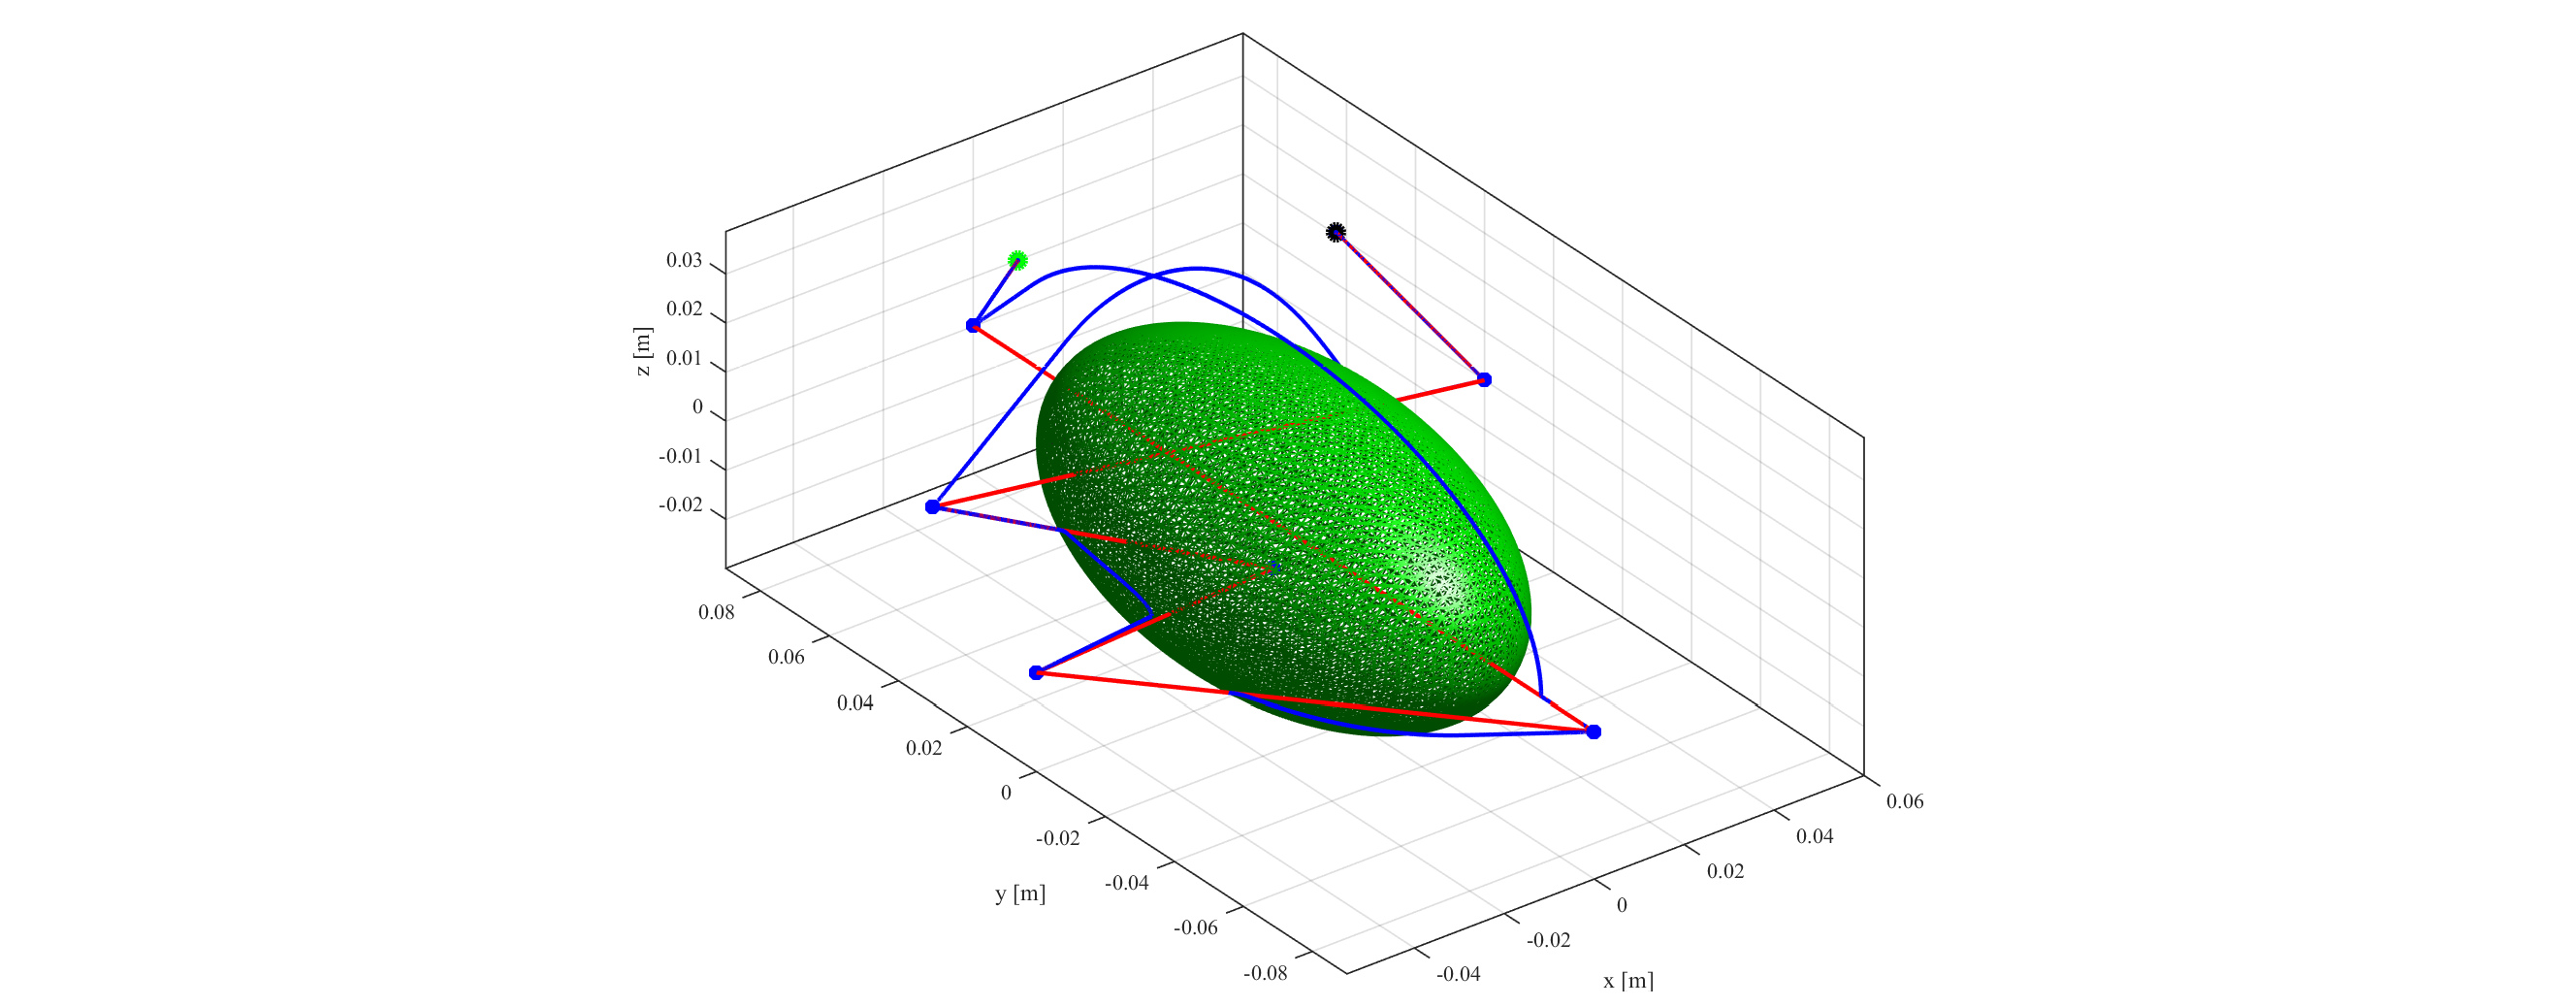
\includegraphics[width=1.4\textwidth]{traj_3d_1.eps}
	\caption{Result of the MATLAB implementation of the safe controller which allows manoeuvring in the euclidean space with an ellipsoid as CBF outlining $\mathcal{X}_u$. The trajectory (blue) along with the immediate trajectory (red) determined from the setpoints given (blue stars). The black circle indicates initial position and the green circle indicates the destination.}
	\label{fig:traj3d_1}
\end{figure}
It is from \autoref{fig:traj3d_1} seen how the controller ensures that the state will never enter the interior of the ellipsoid which indeed was the purpose of the controller. It is also seen how the controller ensures a smooth and elegant detour to reach the desired setpoint while ensuring safety. If a setpoint is given in the interior of $B(\textbf{x})$, the state will settle at the shortest safe distance from that setpoint. It is finally seen how setpoints in the safe area are reached without any problems.

The state trajectory is also plotted in \autoref{fig:traj3d_2} where $x,y,z$ are plotted individually which makes it slightly easier to see the effect of $\sigma(\textbf{x})$. 
\begin{figure}[H]
\centering
	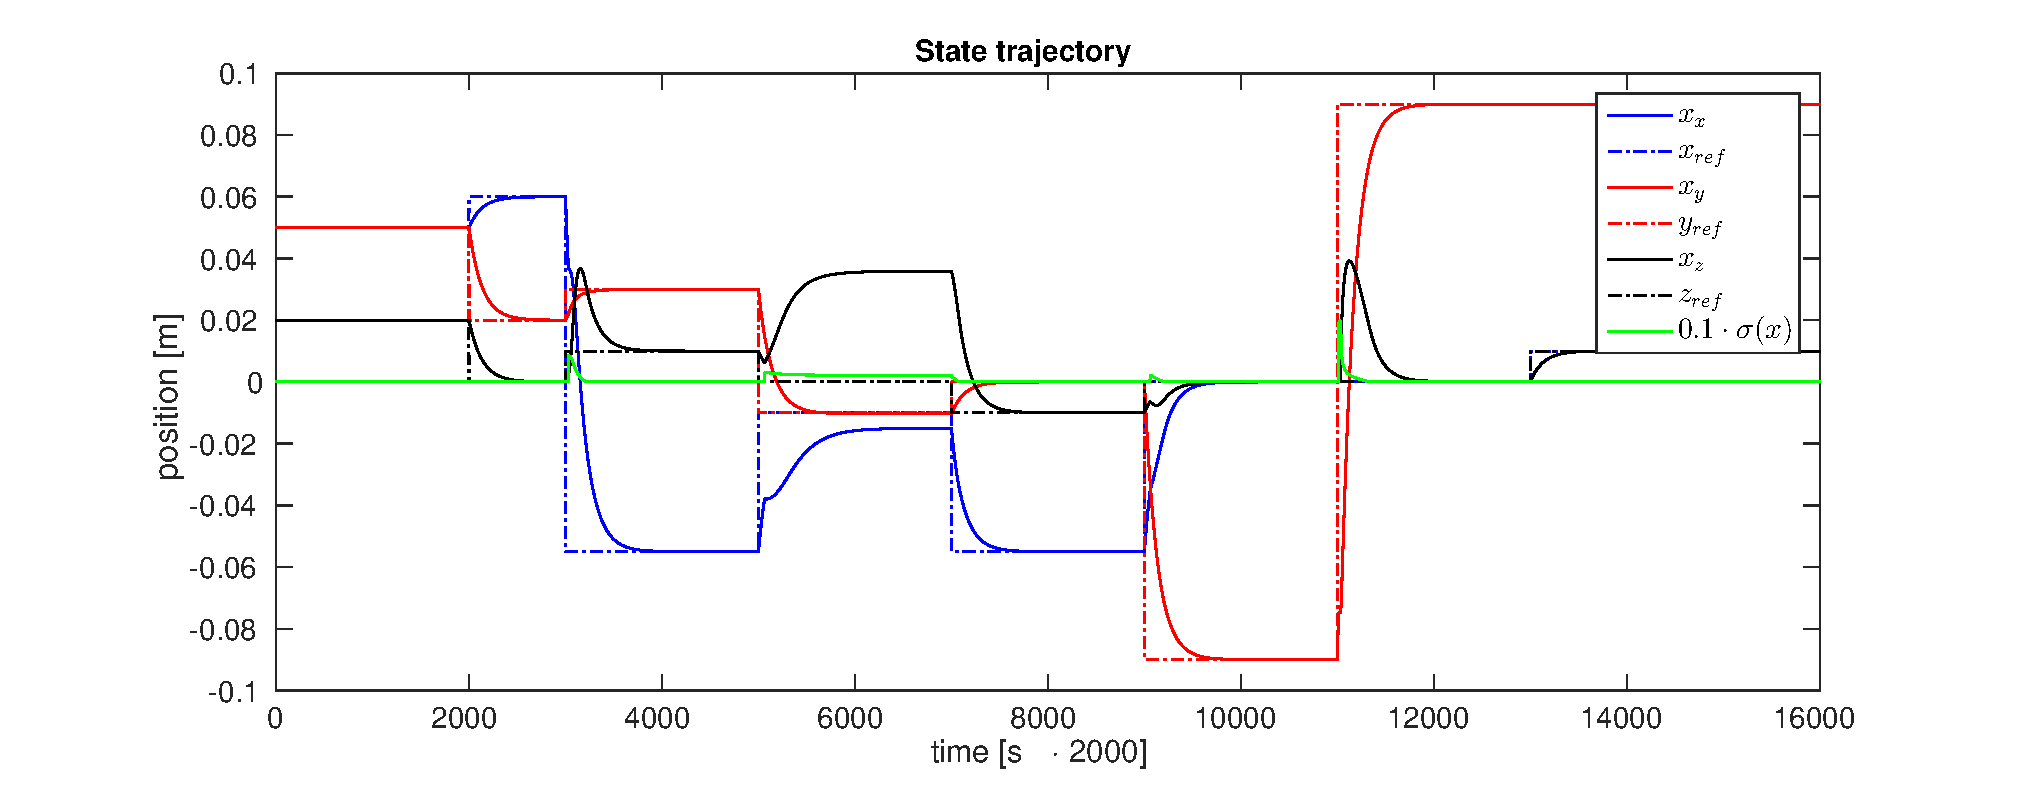
\includegraphics[width=0.9\textwidth]{traj_3d_2.eps}
	\caption{The same trajectory as depicted in \autoref{fig:traj3d_1}. It is here seen how the effect of $\sigma(\textbf{x})$ kicks in when the trajectory approaches the interior of $B(\textbf{x})$ and the position is adjusted accordingly.}
	\label{fig:traj3d_2}
\end{figure}
It is from \autoref{fig:traj3d_2} seen how the effect of $\sigma(\textbf{x})$ kicks in when the trajectory approaches the interior of $B(\textbf{x})$ and the position is adjusted accordingly.

The thickness of 1\,cm, ensured by $\sigma(\textbf{x})$, is visualized in \autoref{fig:traj3d_2:med_sig}.
\begin{figure}[H]
\centering
	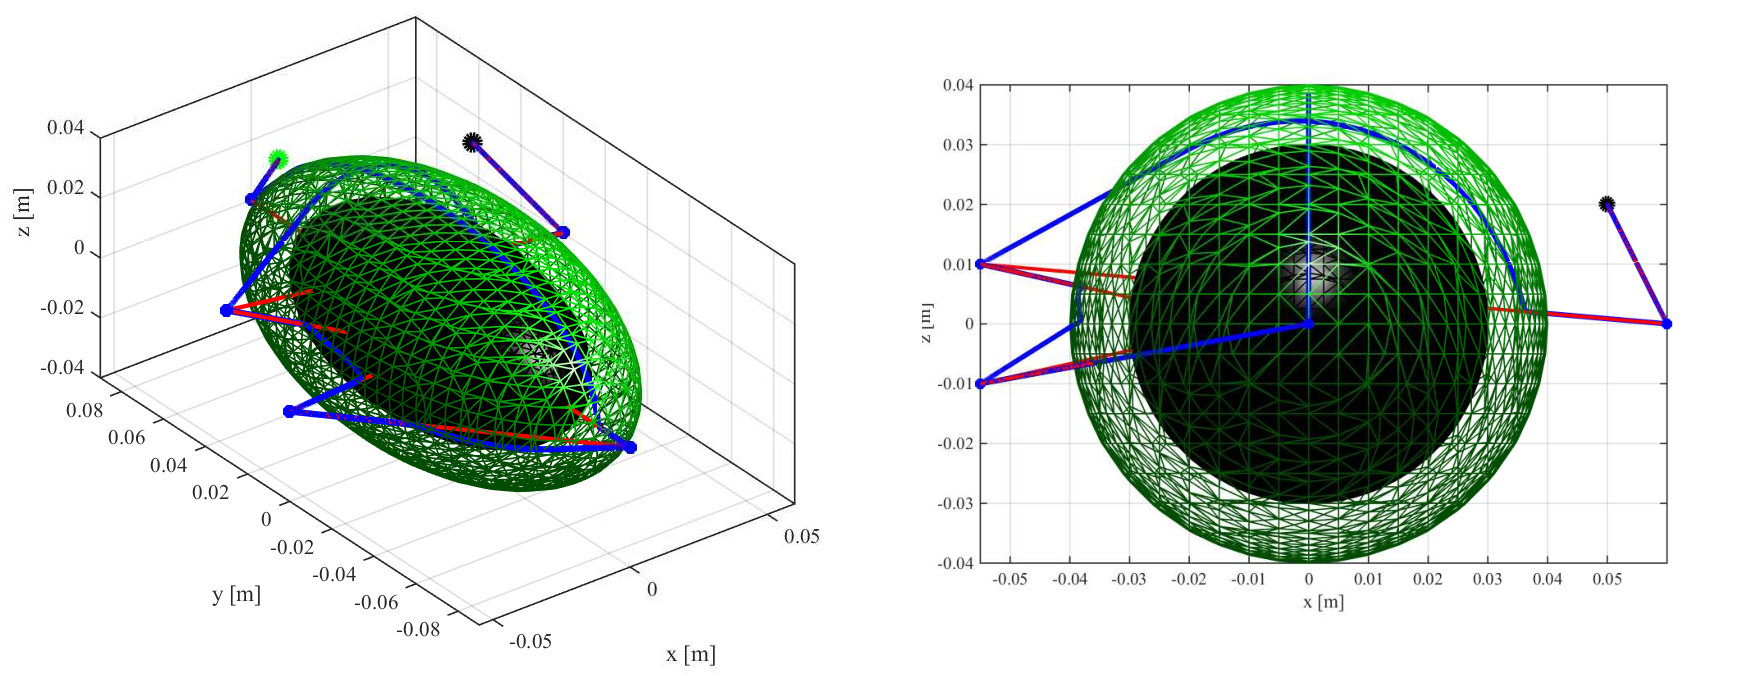
\includegraphics[width=1\textwidth]{traj_3d_med_sigma.pdf}
	\caption{The inner (black) ellipsoid is $\mathcal{X}_u$ and the rim around the inner ellipsoid is $\mathcal{T}$. Thus $\mathcal{X}_0 = \mathcal{X} \backslash \mathcal{X}_u$. The trajectory is initiated from the black circle.}
	\label{fig:traj3d_2:med_sig}
\end{figure}
It is from \autoref{fig:traj3d_2:med_sig} seen that the trajectory starts to be redirected when it enters $\mathcal{T}$ in a smooth manner. The trajectory will always take the shortest safe path.



%It is seen that $L_fB_0(\mathbf{x})$ complies with the relaxed constraint, and hence this candidate barrier function is validated and will be used in the design of the safety controller.

%\newpage
%Based on the modelled decoupled first order systems, identical linear position controllers as in \autoref{eq:utilde} are used for each axis, calculated as presented in \autoref{sec:K_Nbar_1D_1storder}, which results in the closed-loop system on the safe region $\mathcal{X}_0$ on the form
%\begin{equation}\label{eq:3D_sys_static}
%\small
%\dot{\begin{bmatrix}
%	x_x\\x_y\\x_z
%	\end{bmatrix}} =
%\underbrace{\begin{bmatrix}
%	-1/\tau_x & 0 & 0\\0 & -1/\tau_y & 0 \\ 0 & 0 & -1/\tau_z
%	\end{bmatrix}
%	\begin{bmatrix}
%	x_x\\x_y\\x_z
%	\end{bmatrix}}_{f(\mathbf{x})} +
%\underbrace{\begin{bmatrix}
%	1/\tau_x& 0 & 0 \\ 0& 1/\tau_y & 0 \\0& 0& 1/\tau_z
%	\end{bmatrix}}_{g(\mathbf{x})}
%\underbrace{\left(\begin{bmatrix}
%	\bar{\mathbf{N}}_x & 0 & 0 \\0 & \bar{\mathbf{N}}_y & 0 \\0& 0& \bar{\mathbf{N}}_z
%	\end{bmatrix}
%	\begin{bmatrix}
%	x_\text{ref}\\y_\text{ref}\\z_\text{ref}
%	\end{bmatrix}
%	-
%	\begin{bmatrix}
%	\mathbf{K}_x & 0 & 0 \\0 & \mathbf{K}_y & 0 \\0& 0&  \mathbf{K}_z
%	\end{bmatrix}
%	\begin{bmatrix}
%	x_x\\x_y\\x_z
%	\end{bmatrix}\right)}_{\tilde{\mathbf{u}}}
%\end{equation}
%\begin{tabular}{rl}
%where & \\
%$\tau$ & is the time constant given in \autoref{subsec:model_1d}, $\tau = 110$\,ms \textcolor{red}{NEW MEAS!}\\
%$\bar{\mathbf{N}}_i$ & are the system gains for each of the decoupled systems, computed according to \autoref{eq:barm_1}\\
%$\mathbf{K}_i$ & are the controller gains for each of the decoupled systems, computed according to \autoref{eq:K_1}\\
%\end{tabular}\\
%
%\textcolor{red}{pick  values for K and N }
%
%This position controller is used on the safe set $\mathcal{X}_0$, and when the state enters the transition area $\mathcal{T}$ (as defined in \autoref{eq:control_for_safety}) close to the set $\mathcal{X}_u$, the CBF should be used and the two controllers weighted with $\sigma$ as described in \autoref{eq:control_law}. The safe controller or CBF is designed in terms of a valid barrier certificate as defined in \autoref{eq:control_law_safety}, hence a candidate barrier certificate must be constructed.
%
%
%
%
%THIS IS ONLY POSITION, NOT ORIENTATION

%
%Hence, before modelling the system and designing a controller, the kinematics of the AAU da Vinci robot is presented in the following section along with considerations for the definition of the coordinate frames and the transformation between them constituting the kinematic description of the robot.
\section{Implementation of the da Vinci Robot}
\subsection{Kinematics of the AAU da Vinci Robot}
A kinematic description of an object requires defining a right-handed coordinate frame fixed in the object and a coordinate frame fixed in inertial space, the latter which the position and orientation of the object can be described relative to. This relative orientation and position of an object (or the frame $i$ fixed in it) with respect to another frame $j=i-1$ can be described through a transformation matrix $T$, containing the orthonormal rotation matrix $R$ and the translation vector $p$ of the frame origin, as 
\begin{equation}
^j_iT = 
\begin{bmatrix}
^j_iR & ^j_ip\\
0 & 1
\end{bmatrix}, \label{eq:kin_transformation}
\qquad \text{where} \qquad
^j_ip = 
\begin{bmatrix}
a\\b\\d
\end{bmatrix}
\end{equation}
and the simplest rotation matrices $R$ are rotations about a single axis, which can be combined to obtain an arbitrary rotation
\begin{small}
	\begin{equation}
	R_x(\alpha) = 
	\begin{bmatrix}
	1 & 0 & 0\\
	0 & \cos\alpha & -\sin\alpha\\
	0 & \sin\alpha & \cos\alpha
	\end{bmatrix} 
	\qquad
	R_y(\beta) = 
	\begin{bmatrix}
	\cos\beta & 0 & \sin\beta \\
	0 & 1 & 0\\
	-\sin\beta & 0 & \cos\beta
	\end{bmatrix}
	\qquad
	R_z(\theta) = 
	\begin{bmatrix}
	\cos\theta & -\sin\theta & 0\\
	\sin\theta & \cos\theta & 0\\
	0 & 0 & 1
	\end{bmatrix}
	\label{eq:RxRyRz_chapter}
	\end{equation}
\end{small}

For the robotic patient manipulator comprising a number of links, coordinate frames are defined for each degree of freedom, i.e. placed in each joint such that one of the frame axes is the axis of free rotation or translation. The kinematic chain is now the sequence of alternate links and joints starting from the link fixed in inertial space and ending at the tip of the robotic tool. The link preceding a joint is its parent link, while the link succeeding it is its child link. The transformation between any two frames is given as the product of the transformation matrices in the kinematic chain between them. An example of a sequence of transformations can be seen in \autoref{app:kinematic_model_robot}.

For the resolution of frame definitions it is preferred to adapt the  robot coordinate frame convention \gls{dh} because it is one of the most widespread kinematic descriptions in the robot kinematics community, and because it describes transformations between two successive frames in the kinematic chain on a succinct and standardized form
\begin{equation}
\hspace*{-2mm}
\small
^{i-1}_{\phantom{-1}i} T =
\begin{bmatrix}
R_z(\theta_i) & \begin{bmatrix}0\\ 0\\ d_i\end{bmatrix}\\
0 & 1
\end{bmatrix}
\begin{bmatrix}
R_x(\alpha_i) & \begin{bmatrix}a_i\\ 0\\ 0\end{bmatrix}\\
0 & 1
\end{bmatrix}
\label{eq:dh}
\end{equation}
In the \gls{dh} kinematic description each frame is fixed with respect to its parent link, and its $z$-axis is aligned with the actuation axis of its child link. The free rotation/translation always taking place around/along the local $z$ axis, and as seen from \autoref{eq:dh} any fixed or free rotation/translation about/along the $z$-axis is implemented (intrinsically) before any fixed rotation/translation about/along the (new) $x$-axis. For more details on the \gls{dh} convention and robot frames defined according to is, see \autoref{sec:denavit_hartenberg}.

%\begin{itemize}
%	\itemsep-1.3mm 
%	\item variable/parameter $\theta_i$ is the angle from $x_{i-1}$ to $x_i$ about $z_{i-1}$
%	\item variable/parameter $d_i$ is the distance from origin $i-1$ to $x_i$ measured along $z_{i-1}$
%	\item parameter $a_i$ is the distance from $z_{i-1}$ to $z_i$ measured along $x_i$
%	\item parameter $\alpha_i$ is the angle from $z_{i-1}$ to $z_i$ about $x_i$
%\end{itemize}

In the robot description in \gls{ros}, however, the kinematics are described in the \texttt{xacro} files on the form
\begin{equation}
\hspace*{-2mm}
\small
^{i-1}_{\phantom{-1}i}T =
\begin{bmatrix}
R_z(\text{yaw})R_y(\text{pitch})R_x(\text{roll}) & \begin{bmatrix}a_i\\ b_i\\ d_i\end{bmatrix}\\
0 & 1
\end{bmatrix}
\begin{bmatrix}
R_z(\theta_i^*)R_y(\beta_i^*)R_x(\alpha_i^*) & \begin{bmatrix}a_i^*\\ b_i^*\\ d_i^* \end{bmatrix}\\
0 & 1
\end{bmatrix}
\label{eq:xacro_transformation_chapter}
\end{equation}
Here fixed translations are implemented first, then RPY rotations (extrinsic roll (about $x$-axis), pitch (about $y$-axis), yaw (about $z$-axis) rotation), and finally the free rotation or translation (denoted by $^*$ in \autoref{eq:xacro_transformation_chapter}) about/along one of the rotated axes. Furthermore, the convention here is that each frame (joint) is fixed in its child link (corresponding to the fixed rotations preceding the free rotation), and not in its parent link as in the DH convention. The transformation  $^{i-1}_{\phantom{-1}i} T$ is implemented in joint $i$ in the \texttt{xacro} file  as (for joint 8)
\begin{lstlisting}[language=xml]
<joint name="p4_hand_pitch"  type="revolute">
<origin
xyz="0 0 0"
rpy="1.5708 0 0" />
<parent link="rcm_vitual0" />
<child link="rcm_vitual1" />
<axis xyz="0 0 1" />
...
</joint>
\end{lstlisting}

A compromise is made, defining a new set of frames for the da Vinci kinematics, adhering to the \gls{dh} constraint that each free rotation/translation is about/along the local $z$-axis. The new kinematic frames are visualized in \autoref{fig:p4_hand_compromise_frames_chapter}, the parameters listed in table \ref{tab:new_kin_short}. Furthermore, for simplification of the inverse kinematics solver, the two passive joints mimicking the hand pitch movement are removed from the existing kinematic chain, visualized in \autoref{fig:p4_hand_xacro_frames_chapter}, and parameters listed in table \ref{tab:old_kin_short} for comparison.  



\begin{table}[htbp]
	\small
	\centering
\subbottom[Old robot hand kinematics including mimicking joints, corresponding to \autoref{fig:p4_hand_xacro_frames_chapter}.]{%
	\begin{tabular}{r | rrr | ccc | c l}\hline
		& \multicolumn{3}{c|}{fixed translation  [m]} & \multicolumn{3}{c|}{fixed rotation [rad]} & freedom & \\
		frame  & $a$ ($x$)  & $b$ ($y$)  & $d$ ($z$)  & roll  & pitch & yaw & $\alpha^*, \beta^*, \theta^*$ or $d^*$ & joint name\\\hline
		7 & -0.042 & 0 & 0.161 & 0 & 0 & 0 & $\phantom{-}\alpha_7^*$ & \texttt{hand\_roll} \\
		8 & 0 & 0 & 0 & 0 & -0.288 & 0 & $-\beta_8^*$ & \texttt{hand\_pitch} \\
		9 & 0.011 & 0 & 0.186 & $\pi$ & 0.288 & 0 & $\phantom{-}\beta_8$ & mimic \texttt{hand\_pitch} \\
		10 & 0.520 & 0 & 0 & $\pi$ & 0& 0 &  $-\beta_8$ & mimic \texttt{hand\_pitch} \\
		11 & 0 & 0 & -0.120  & 0 & 0 & 0 & $\phantom{-}d_{11}^*$ & \texttt{instrument\_slide} \\
		12 & 0.052 & 0 & 0 & $\pi$ & 0 & $\pi/2$ & $\phantom{-}\theta_{12}^*$ & \texttt{instrument\_roll} \\
		13 & 0 & 0 & 0.177 & 0 & 0 & 0 & $-\alpha_{13}^*$ & \texttt{instrument\_pitch} \\
		14L & 0 & 0 & 0.009 & $\pi/2$ & $\pi/2$ & 0 & $-\theta_{14L}^*$ & \texttt{instrument\_jaw\_left} \\
		14R & 0 & 0 & 0.009 & $\pi/2$ & $\pi/2$ & 0 & $\phantom{-}\theta_{14R}^*$ & \texttt{instrument\_jaw\_right} \\
	\end{tabular}\label{tab:old_kin_short}}
	\vspace*{1mm}
\subbottom[New robot hand kinematics excluding mimicking joints, corresponding to \autoref{fig:p4_hand_compromise_frames_chapter}.]{%
	\begin{tabular}{r | rrr | ccc | c l}\hline
		& \multicolumn{3}{c|}{fixed translation  [m]} & \multicolumn{3}{c|}{fixed rotation [rad]} & freedom & \\
		frame  & $a$ ($x$)  & $b$ ($y$)  & $d$ ($z$)  & roll  & pitch & yaw & $\theta^*$ or $d^*$ & joint name\\\hline
		7 & 0.482 & 0 & 0.047 & 0 & $\pi/2$ & 0 & $\theta_7^*$ & \texttt{hand\_roll} \\
		8 & 0 & 0 & 0 & $\pi/2$ & 0 & 0 & $\theta_8^*$ & \texttt{hand\_pitch} \\
		9 & 0.097 & 0 & 0 & 0 & $-\pi/2$ &  0 & $d_9^*$ & \texttt{instrument\_slide} \\
		10 & 0 & 0 & 0 & 0 & 0 & 0 & $\theta_{10}^*$ & \texttt{instrument\_roll} \\
		11 & 0 & 0 & 0 & 0 & $\pi/2$ & 0 & $\theta_{11}^*$ & \texttt{instrument\_pitch} \\
		12L & 0.009 & 0 & 0 & $-\pi/2$ & 0 & 0 & $\theta_{12L}^*$ & \texttt{instrument\_jaw\_left} \\
		12R & 0.009 & 0 & 0 & $-\pi/2$ & 0 & 0 & $\theta_{12R}^*$ & \texttt{instrument\_jaw\_right} \\
		\end{tabular}\label{tab:new_kin_short}}
	\caption{Parameters and variables (marked with $^*$) for the robot kinematic description implemented in \gls{ros} and visualized in \autoref{fig:robot_hand_kinematics}. Free angles are named with $\alpha$ being a rotation about the $+x$-axis, $\beta$ about the $+y$-axis and $\theta$ about the $+z$-axis.}
	\label{tab:xacro_param_short}
\end{table}



\begin{figure}[htbp]
\hspace*{-15mm}
\begin{minipage}{1.15\textwidth}
	\subbottom[Old robot hand kinematics including mimick joints, parameters given in table \ref{tab:old_kin_short}.]{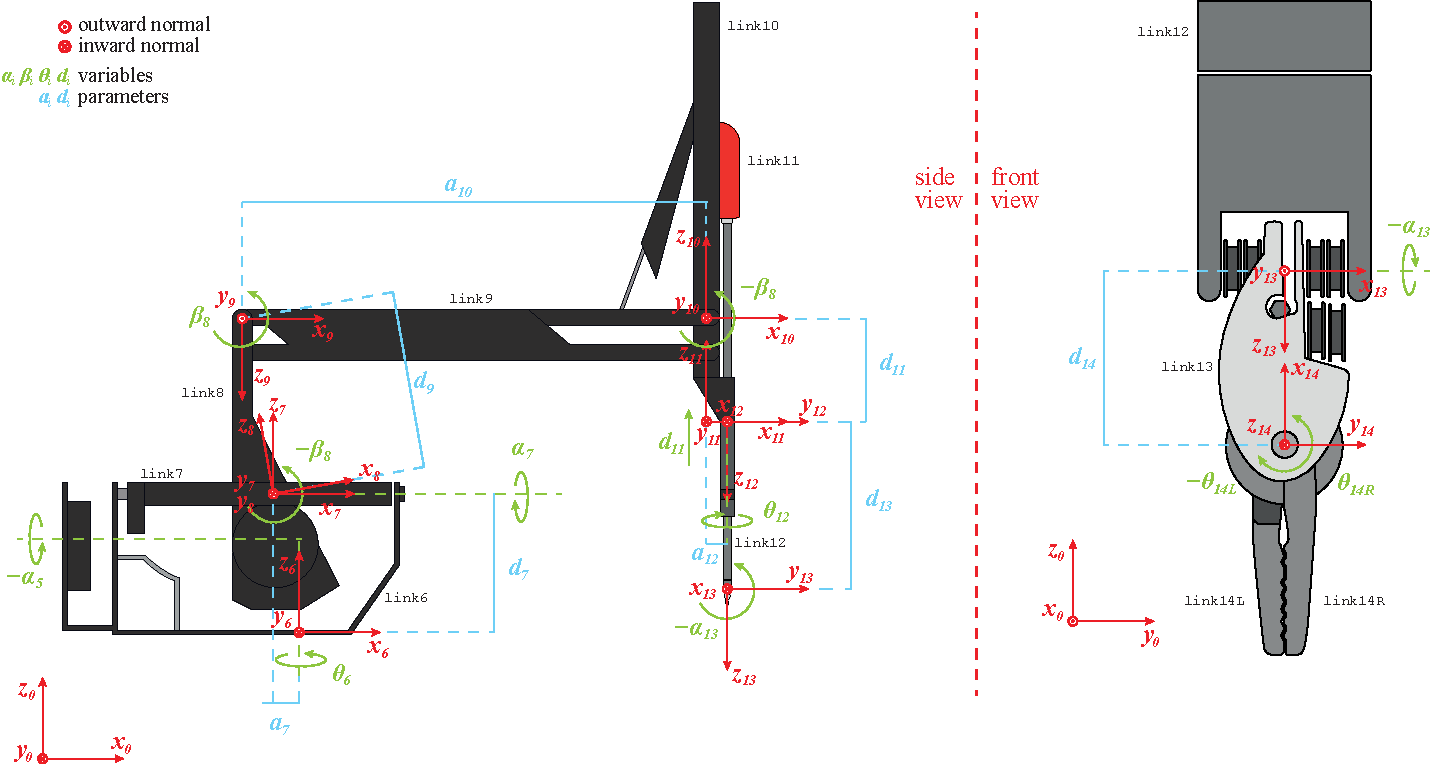
\includegraphics[width=\textwidth]{p4_hand_xacro_frames_chapter.pdf}\label{fig:p4_hand_xacro_frames_chapter}}%
	\vspace*{5mm}
	\subbottom[New robot hand kinematics excluding mimick joints, parameters given in table \ref{tab:new_kin_short}.]{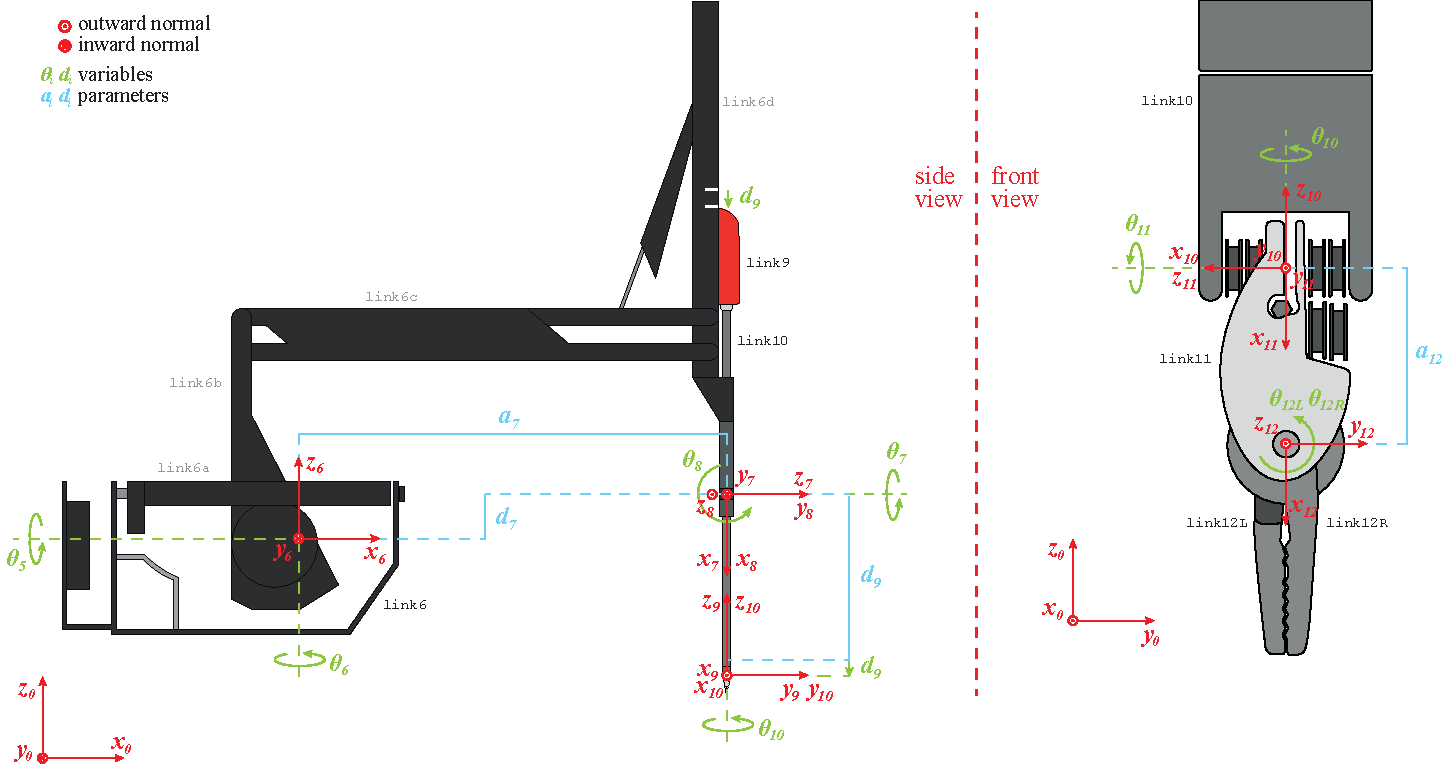
\includegraphics[width=\textwidth]{p4_hand_compromise_frames_chapter.pdf}\label{fig:p4_hand_compromise_frames_chapter}}%
	\caption{Orientation and position of coordinate frames $\Psi_7$, $\Psi_8$, etc. corresponding to the controllable joints of the robotic patient manipulator.  For convenience of placing the hand roll and pitch frames in the pivot point in the new kinematic description in \autoref{fig:p4_hand_compromise_frames_chapter}, a virtual link is inserted in the \texttt{xacro} file after each of these two joints.}
	\label{fig:robot_hand_kinematics}
\end{minipage}
\end{figure}
For more details on the original and new kinematic descriptions implemented in \gls{ros}; including all measurements of parameters, gearing ratios, code for testing the kinematic description in Matlab, and measurements of distances for different configurations; please refer to \autoref{sec:existing_kinematics} and \ref{sec:app_activejoints_kinematics} in \autoref{app:kinematic_model_robot}.










\subsection{Employing Inverse Kinematics for a Controller in 3D Cartesian Space}
The controller presented in this chapter is developed for 3D position and orientation control of the tool tip, and hence relies on the use of inverse kinematics for the (ambiguous) mapping from 3D Cartesian space to 6D joint space. The inverse of the kinematic transformation matrix presented in \autoref{eq:kin_transformation} is
\begin{equation}
^j_iT^{-1} = 
\begin{bmatrix}
^j_iR^T & -^j_iR^T\,\,^j_ip\\
0 & 1
\end{bmatrix}
\end{equation}
With the sequence of transformations from frame $k$ to frame $i$ being represented by the transformation matrix $^k_i T$, the inverse transformation, from frame $i$ to frame $k$, is then its matrix inverse $^k_i T^{-1}$
\begin{equation}
^k_iT = ^k_jT \,\, ^j_iT =
\begin{bmatrix}
^k_jR \,\, ^j_iR & ^k_jp+^k_jR \,\, ^j_ip\\
0 & 1
\end{bmatrix}
\qquad \Leftrightarrow \qquad
^k_iT^{-1} = 
\begin{bmatrix}
^j_iR^T\,\, ^k_jR^T & -\,^j_iR^T\,\, ^k_jR^T\,\,^k_jp -\, ^j_iR^T\,\, ^j_ip\\
0 & 1
\end{bmatrix}
\end{equation}
A mapping from six to three degrees of freedom is a surjective map, i.e. several elements in the 6D domain may map to the same element in the 3D co-domain. However the inverse map from 3D to 6D is neither injective nor surjective, as each element in the 3D domain can map to several elements in the 6D co-domain, and hence the mapping requires a decision of the "best" map.

In practice this mapping from the desired 3D Cartesian space configuration to a prudent 6D joint space position of the da Vinci robotic patient manipulator is handled by the \gls{kdl} inverse kinematics solver. Then the transformed joint position commands are passed to the low level controllers (see \autoref{fig:overview}).

The \gls{ik} \gls{kdl} solver employed in \gls{ros} utilizes the kinematic chain from the URDF, which is generated from the \texttt{xacro} link and joint kinematic description as presented in %\autoref{app:kinematic_model_robot}, the model implemented in ROS defined in
\autoref{sec:app_activejoints_kinematics}. From this chain (\texttt{my\_chain} in the below example) a \gls{fk} position solver is created along with an \gls{ik} velocity solver in order to define the \gls{ik} position solver:

\begin{lstlisting}[language=xml]
//Create solver based on kinematic chain
KDL::ChainFkSolverPos_recursive fksolver(my_chain);
KDL::ChainIkSolverVel_pinv iksolverv(my_chain);
KDL::ChainIkSolverPos_NR iksolver = KDL::ChainIkSolverPos_NR(my_chain,fksolver,iksolverv,100,1e-6);

KDL::JntArray q(my_chain.getNrOfJoints());
KDL::JntArray q_init(my_chain.getNrOfJoints());

//Set destination frame
double x, y, z;
std::cout << "Set end-effector position <x y z>:" << std::endl;
std::cin >> x >> y >> z;
KDL::Vector dest_pos(x,y,z);
KDL::Frame dest_frame(dest_pos);

// Compute!
int ret = iksolver.CartToJnt(q_init,dest_frame,q);
\end{lstlisting}

The \gls{kdl} \gls{ik} position solver uses the Newton-Raphson iterative numerical technique through the function \texttt{CartToJnt} to determine a prudent joint configuration implementing the desired Cartesian configuration (given as \texttt{dest\_frame} in the above example). In the above example the initial guess \texttt{q\_init} of the joint configuration is the current joint configuration, and hence care should be taken to only command small changes in configuration for the sake of fast convergence of the \gls{ik} solution.


Three dimensional positions of the tool tip is described in a frame oriented as the inertial frame and offset such that a robot configuration with all free angles and slide set to zero equals a position of the tool tip in [0,0,0].


\section{Conclusion for Safety in the Euclidean Space}
only position, not orientation

